\section{Segmentation}
\label{sec:segmentation}

\begin{figure}[!h]
    \centering
    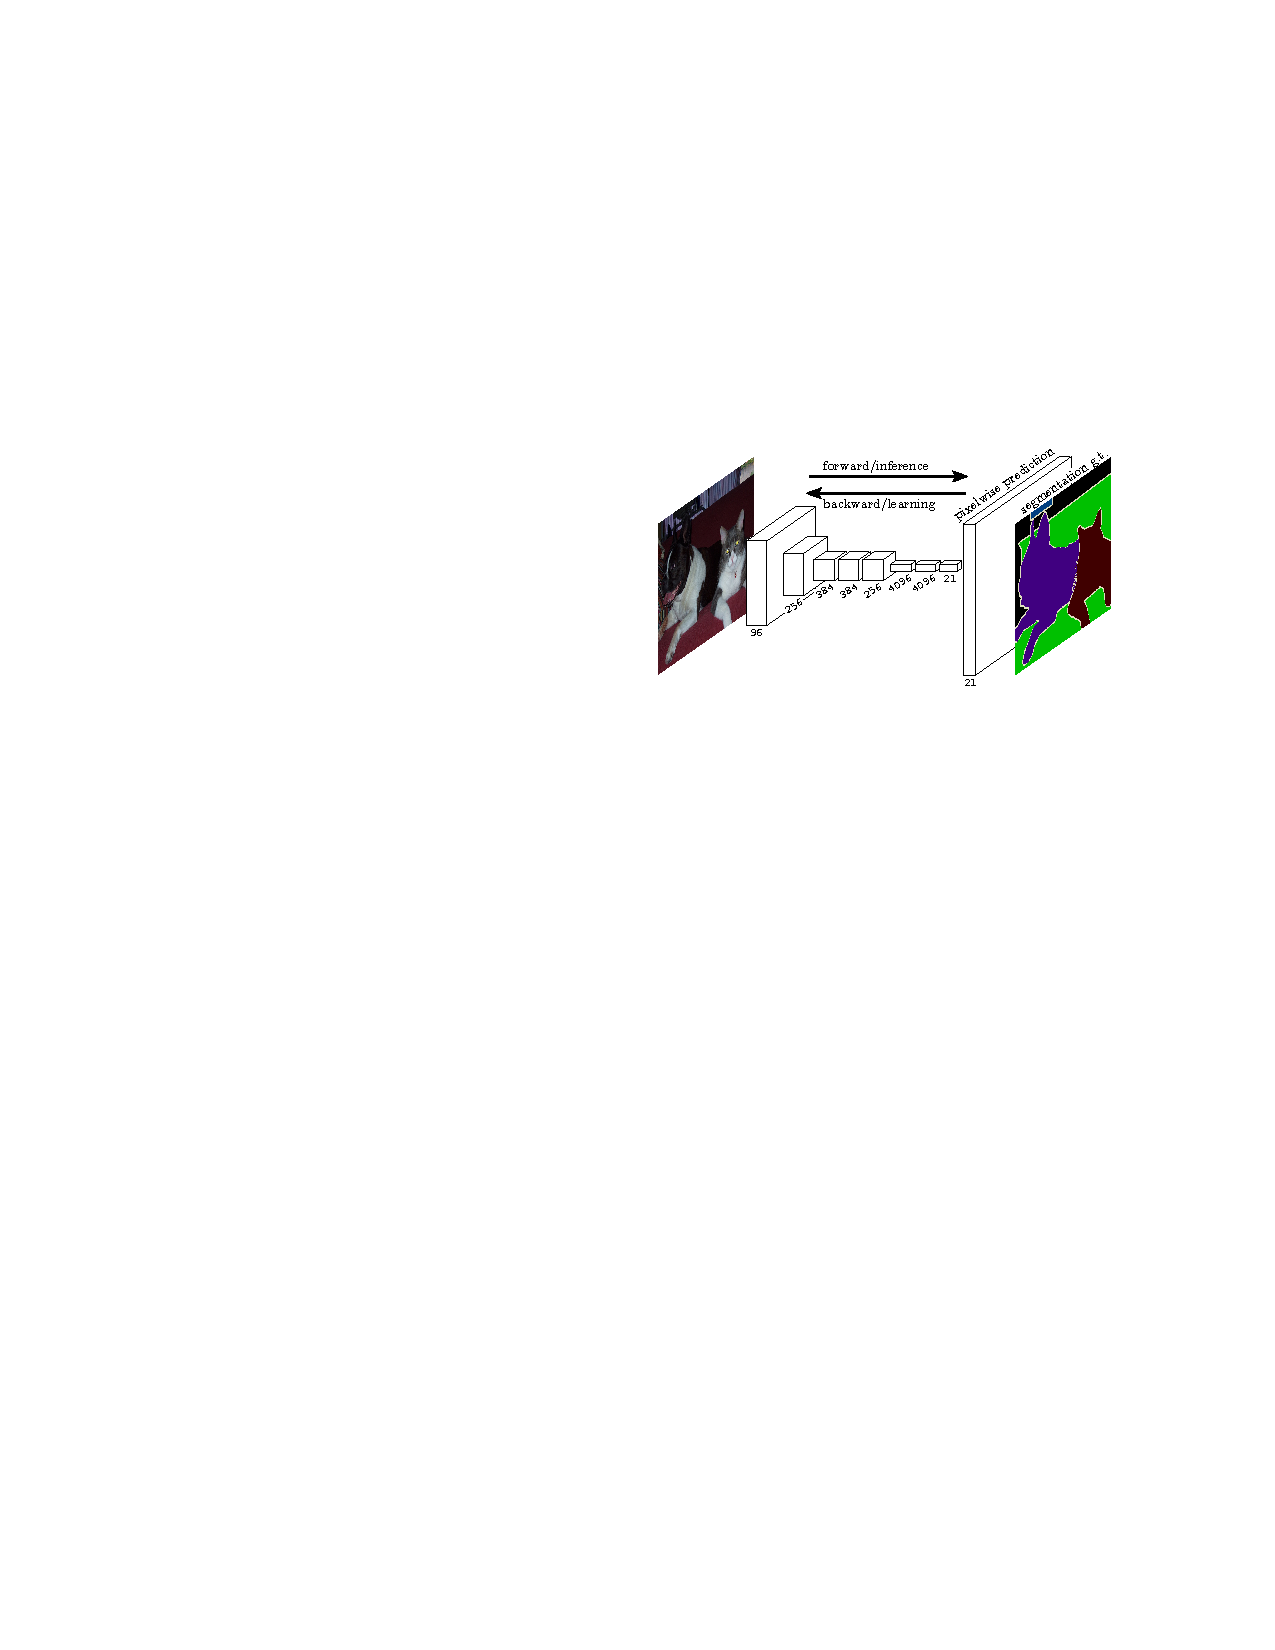
\includegraphics[width=\textwidth]{content/resources/new_images/related_works/fcn.pdf}
    \caption{Fully Convolutional Networks Architecture}
    \label{fig:fcn}
\end{figure}

Segmentation is one of the most important tasks in image processing and has a long history of development. It has grown strongly since neural networks and computing resources starting to explode. One of the basic ideas behind segmentation is that you can use convolution layers as a feature extraction mechanism. By downsampling the input image after passing it through a backbone CNN model containing multiple pooling layers, you can generate a prediction at a smaller scale that needs to be upsampled to the original image size. This approach, which uses fully convolutional layers to perform classification for each pixel in the feature map, is known as Fully Convolutional Networks (FCNs)\cite{FCN}.


The reason behind this architecture that combine deep semantic information in deeper layers and spatial information in shallow layers together. However, there are still many limitations, such as losing spatial information in the downsampling process; its inability to leverage global context information; and the lack of a mechanism for variant-scales.

\begin{figure}[h]
    \centering
    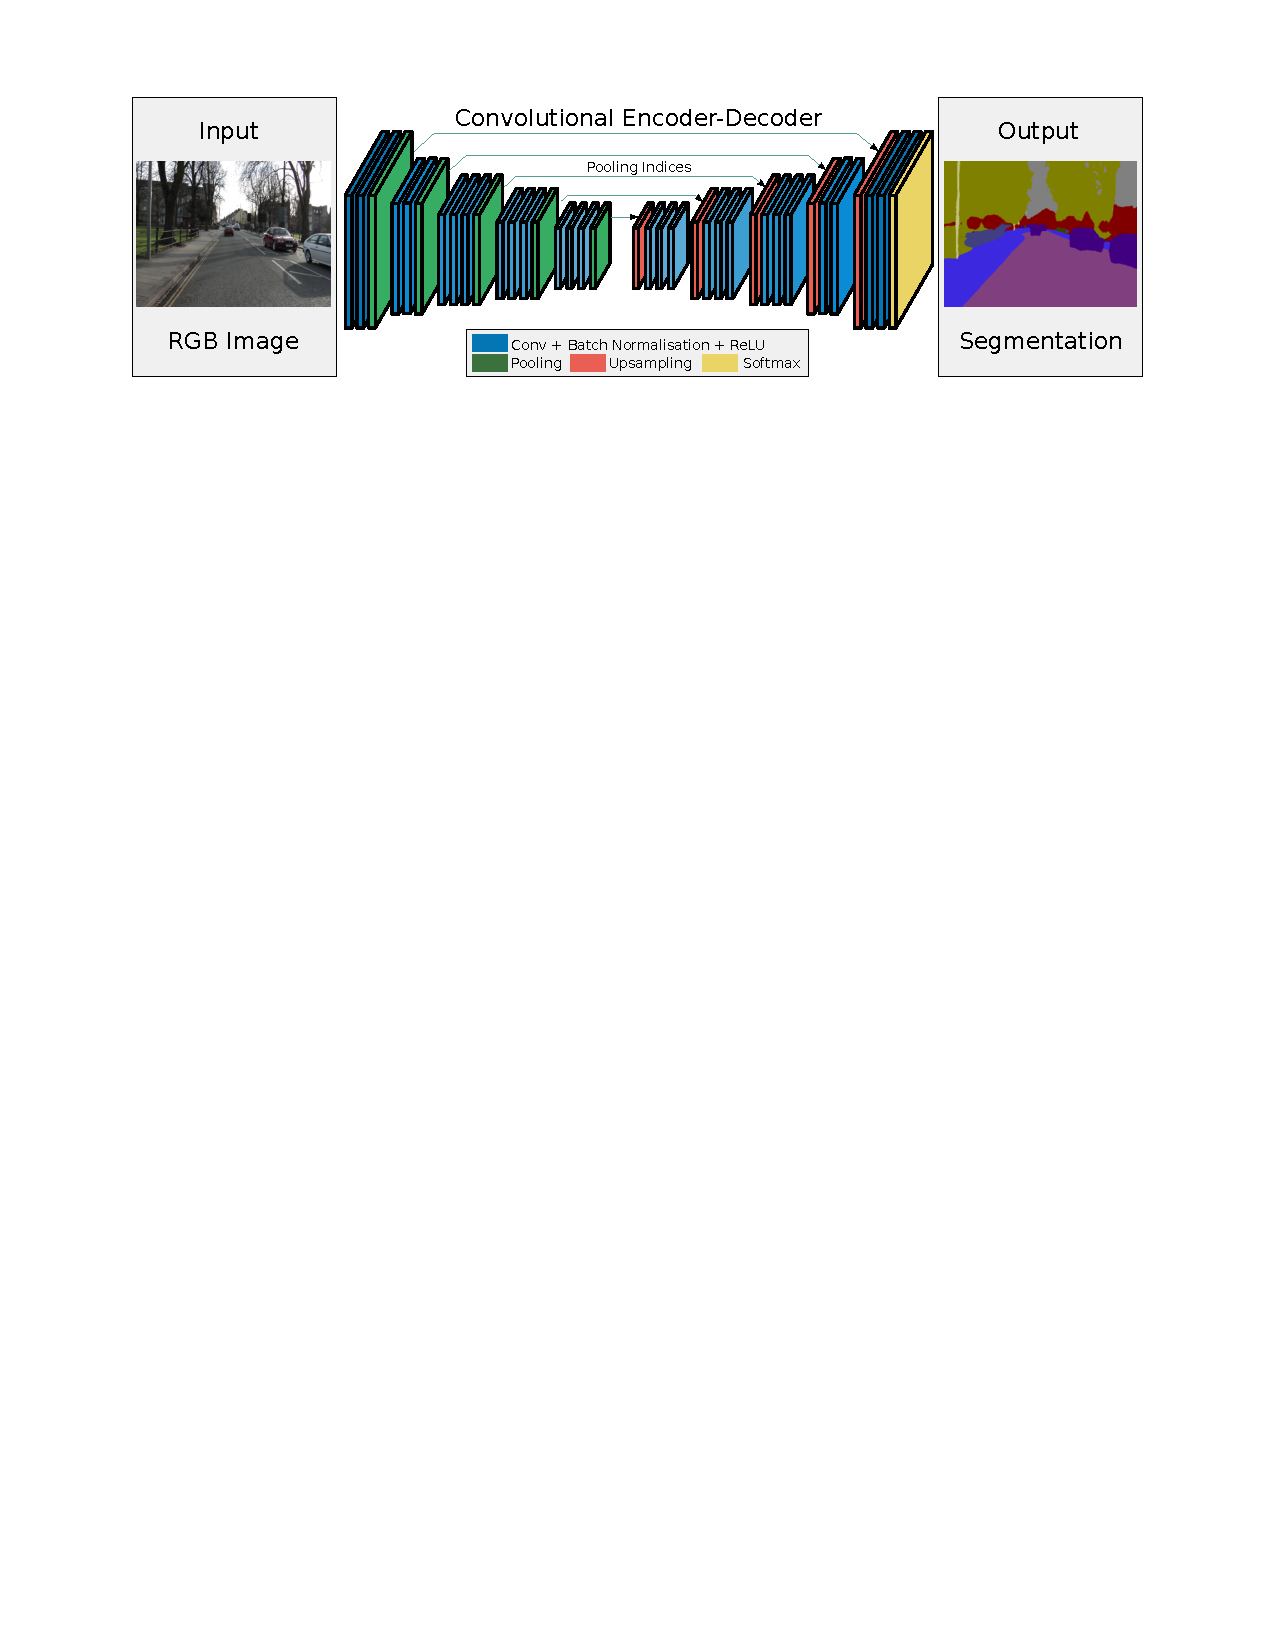
\includegraphics[width=\textwidth]{content/resources/new_images/related_works/segnet.pdf}
    \caption{SegNet Architecture}
    \label{fig:segnet}
\end{figure}

The next popular method is using encoder and decoder based architecture. Segnet\cite{segnet} is the pioneer when do a symmetric architecture between encoder and decoder. In details, decoder mirror copy of the decoder and augment with information from encoder. There are multi descendants inspire from this and popular nowadays like Unet\cite{Unet}

\begin{figure}[h]
    \centering
    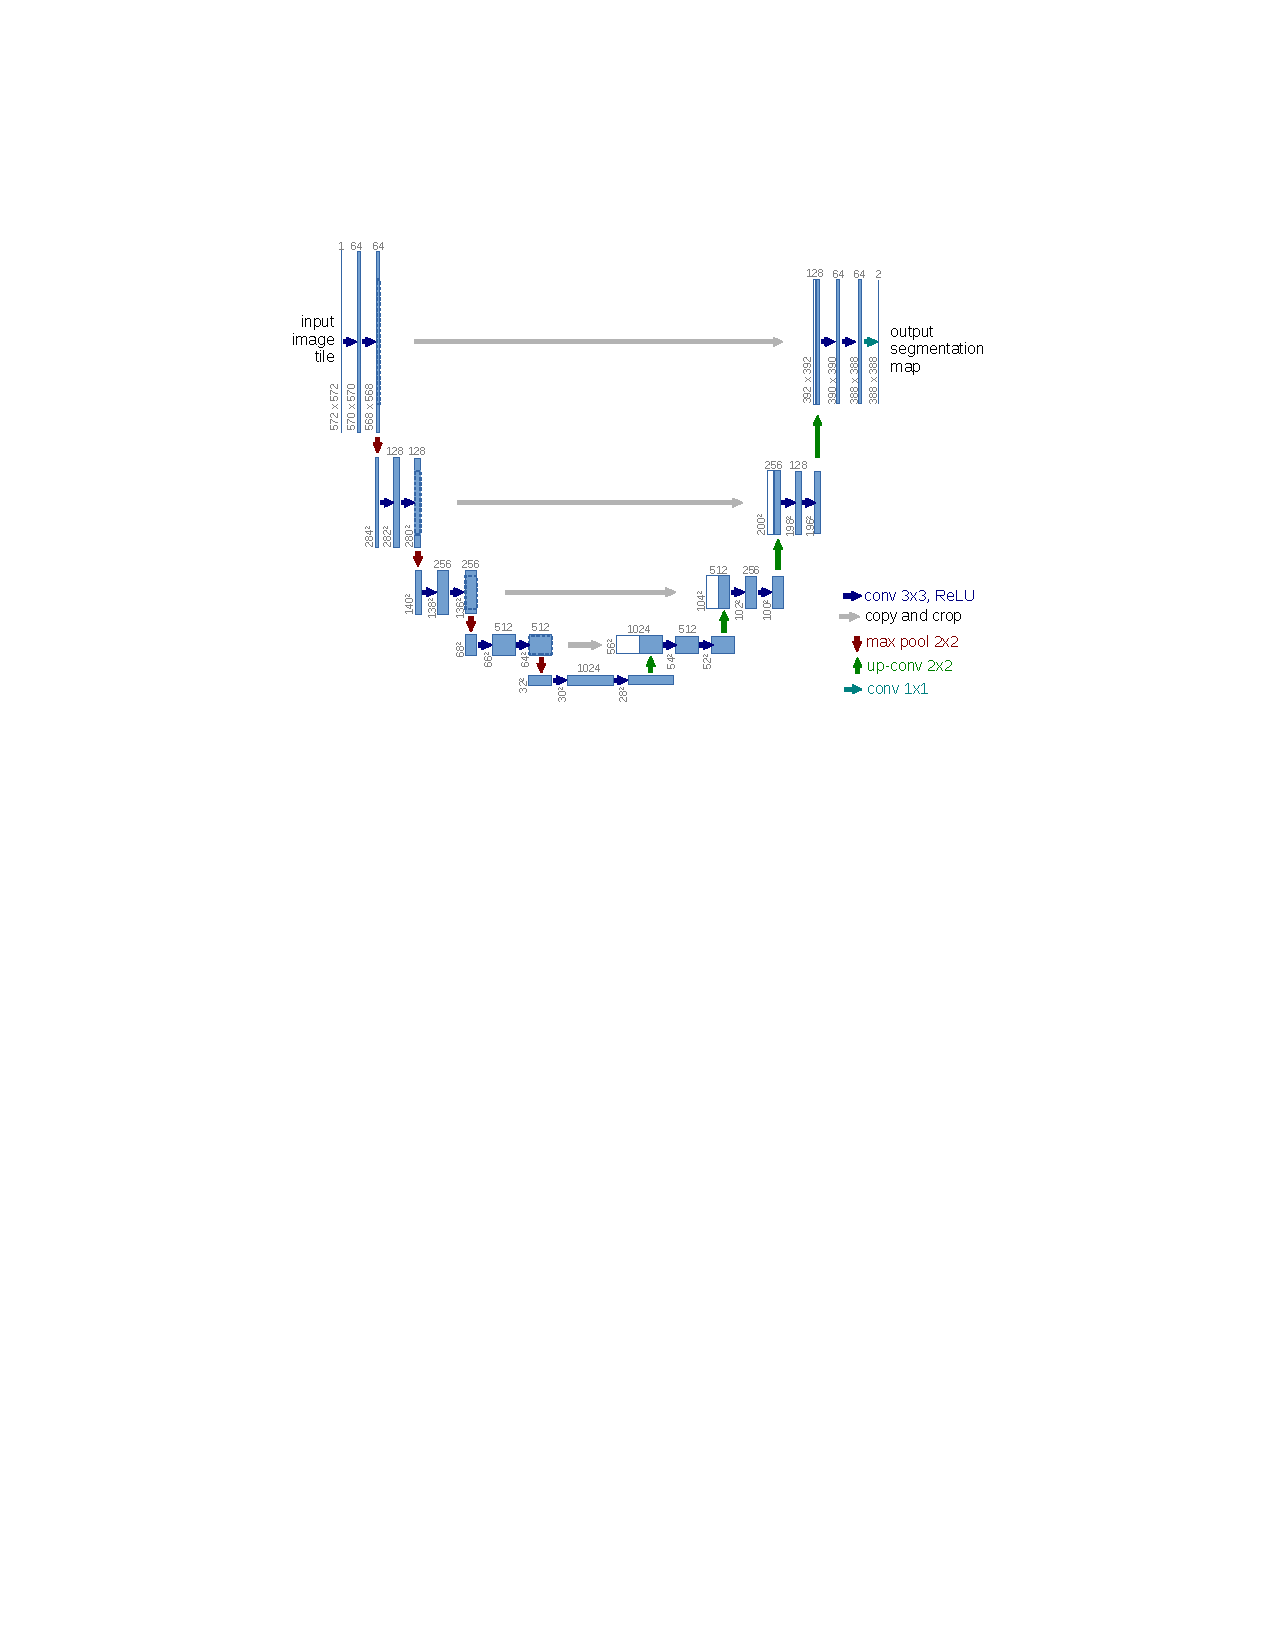
\includegraphics[width=\textwidth]{content/resources/new_images/related_works/unet.pdf}
    \caption{Unet Architecture}
    \label{fig:unet}
\end{figure}

Unet\cite{Unet} is one of the most popular architectures in computer vision, and it has been shown to be very effective in medical applications. The encoder provides spatial information that helps to decode the features more accurately. There are variants of Unet that have been developed specifically for better performance, such as Unet++\cite{UnetPP} and Attention U-Net\cite{AttUnet}. These variants continue to show promise for semantic segmentation tasks, with improved accuracy over other methods.

\begin{figure}[h]
    \centering
    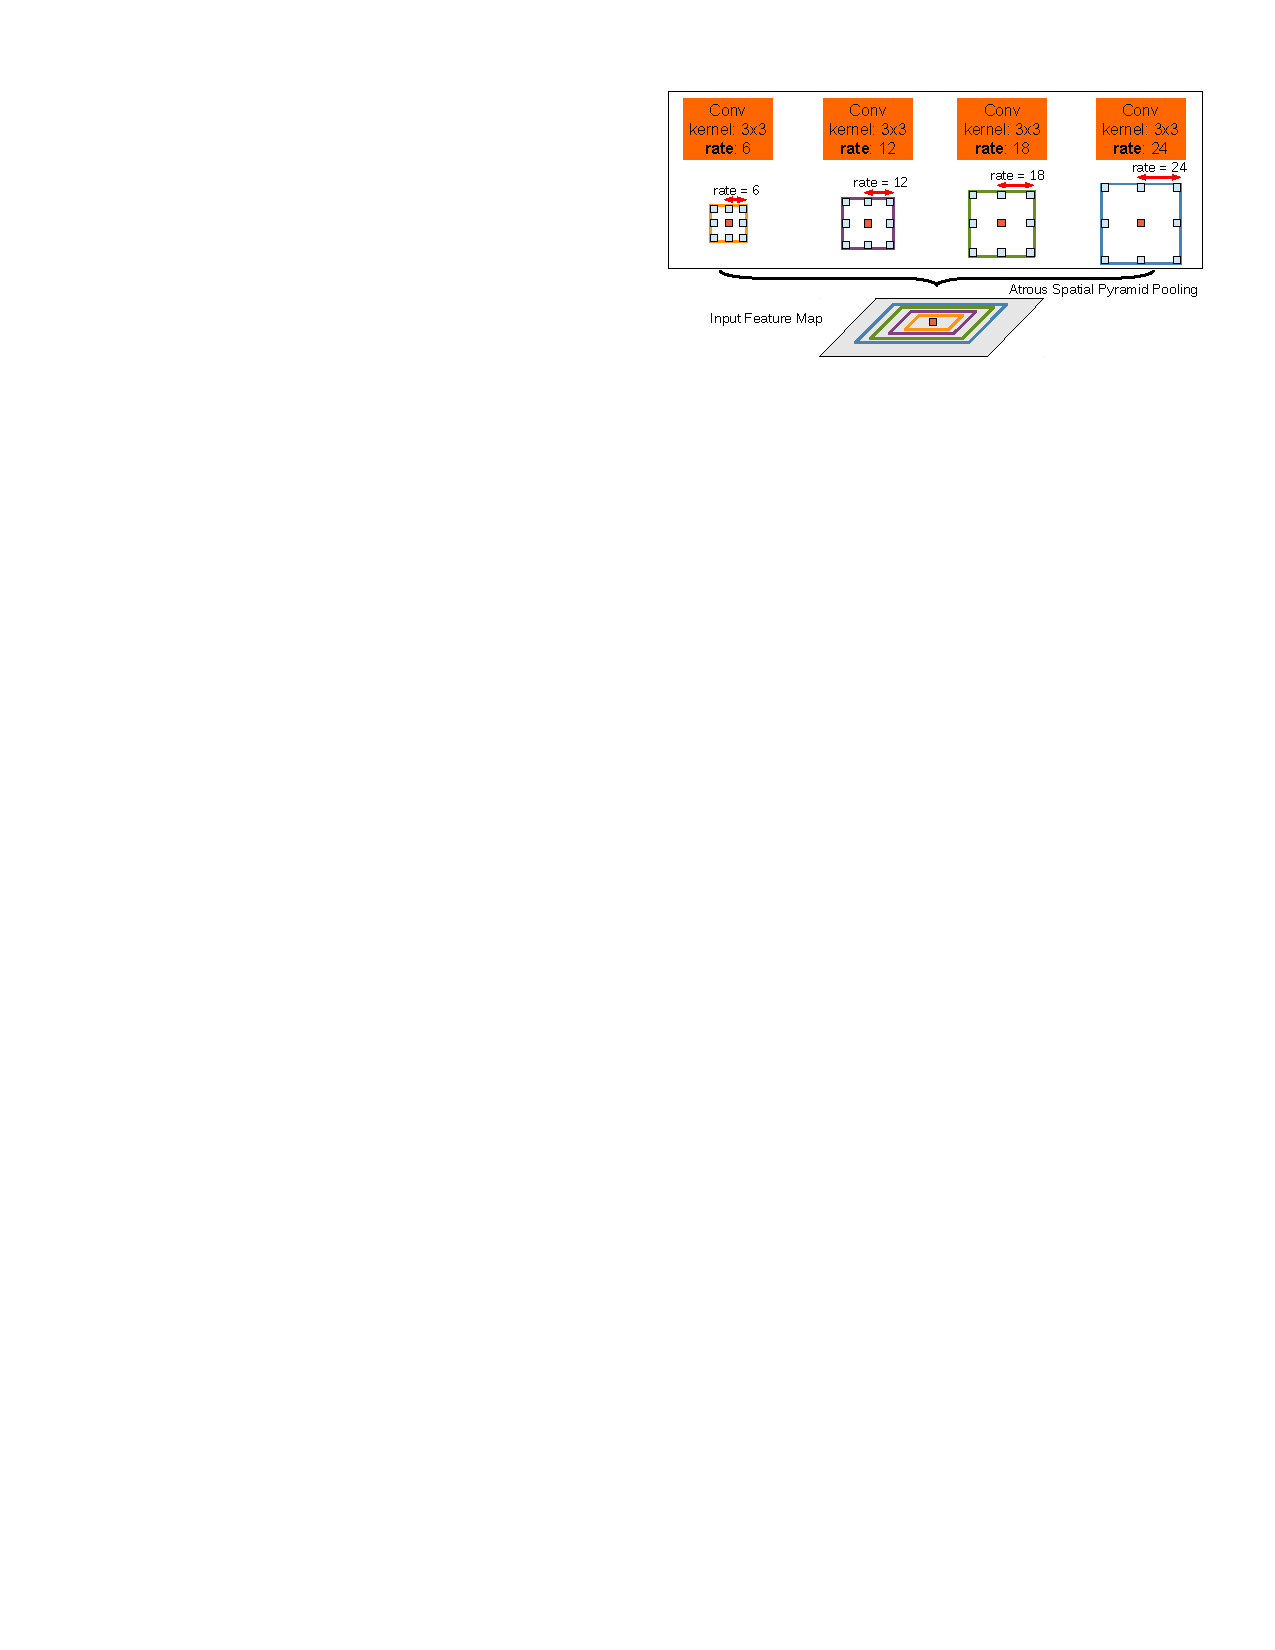
\includegraphics[width=\textwidth]{content/resources/new_images/related_works/aspp.pdf}
    \caption{Atrous Spatial Pyramid Pooling}
    \label{fig:unet}
\end{figure}

Another model to approach the fixed kernel size problem is of the family of segmentation models called DeepLab\cite{Deeplab}. DeepLab model family is a promising solution to the fixed kernel size problem. They use dilated convolution (also known as atrous convolution) to learn features from a larger region without increasing computational expenses. This allows for deeper neural networks, which can better capture complex patterns in data. Atrous Convolutions with different rates are stacked in the encoder, called the Atrous Spatial Pyramid Pooling module. This module offers the ability to learn multi-scale features in the encoding phase, which is important for accurately capturing information about objects and scenes.

\begin{figure}[h]
    \centering
    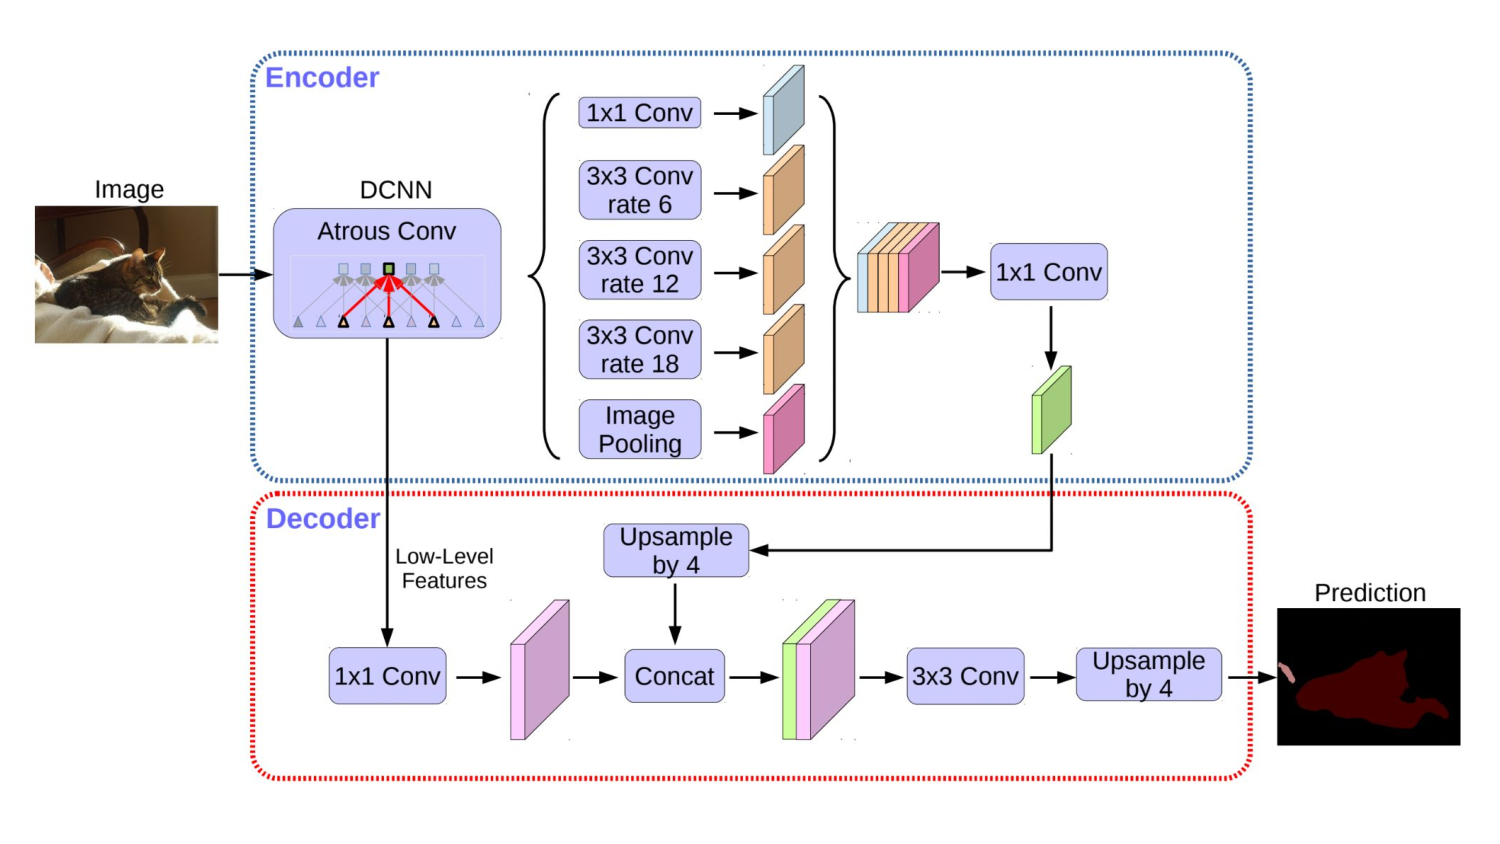
\includegraphics[width=\textwidth]{content/resources/new_images/related_works/deeplabv3.pdf}
    \caption{DeepLabv3 Architecture}
    \label{fig:deeplabv3}
\end{figure}

Computer vision has come a long way in the past few years. Researchers have found that transformer power is one of the potential ways to improve computer vision. Transformers are famous for their ability in downstream task in natural language processing. However, the naive usage that replaces transformer vision as a feature extraction is not exploiting almost its capability. Due to that TransUnet\cite{TransUnet} use the strong point of them ideas, which is transformer leverage both detailed high-resolution spatial information from CNN features and the global context encoded by Transformers, also inspired by the u-shaped architectural design 

\begin{figure}[h]
    \centering
    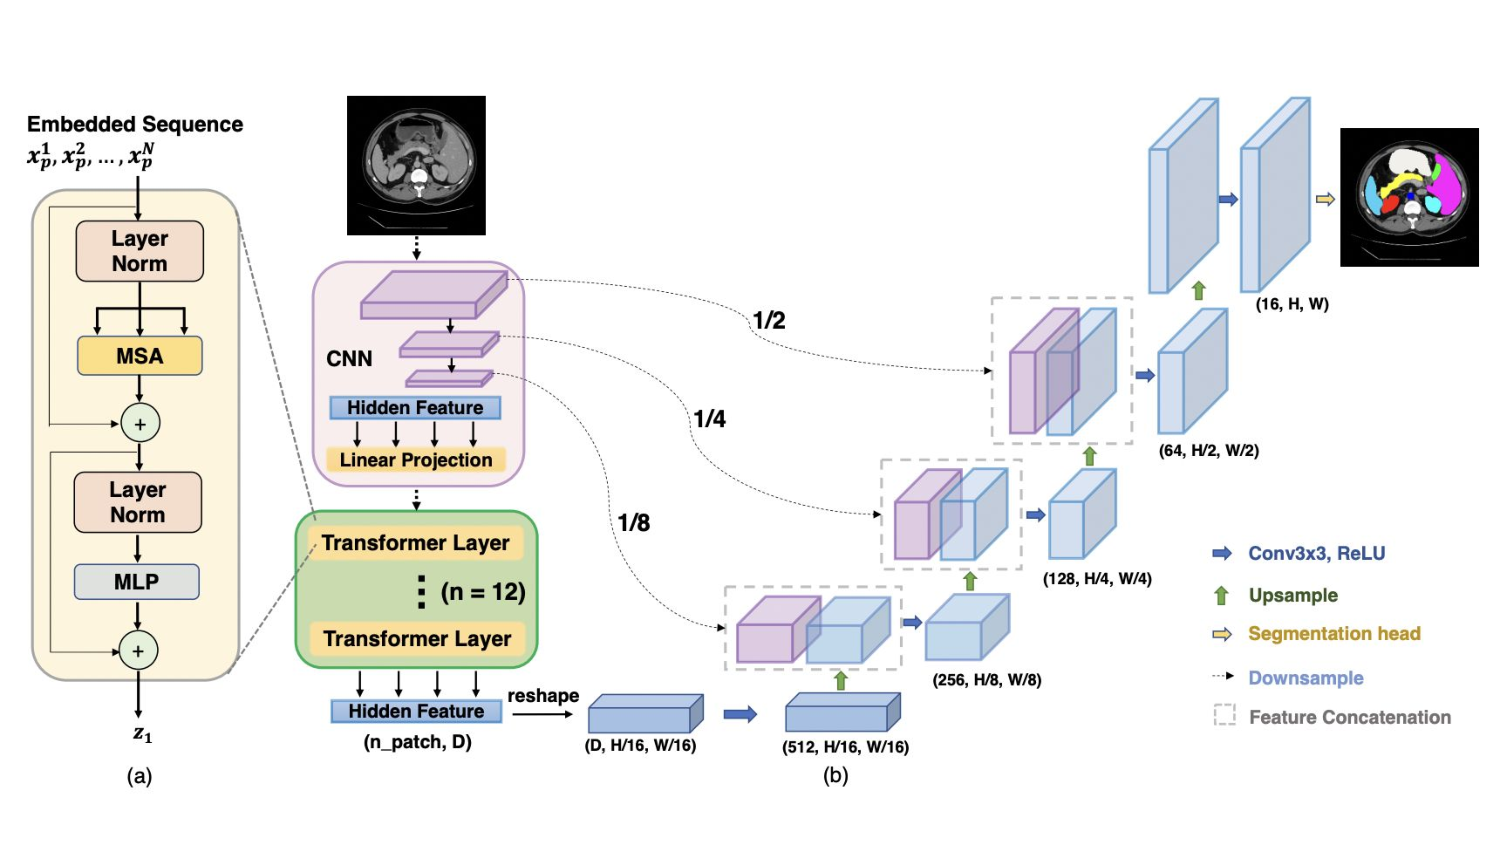
\includegraphics[width=\textwidth]{content/resources/new_images/related_works/transunet.pdf}
    \caption{(a) schematic of the Transformer layer; (b) architecture of the TransUNet}
    \label{fig:transunet}
\end{figure}